% Chapter 2

\chapter{Data Analysis} % Main chapter title

\label{Chapter2} % For referencing the chapter elsewhere, use \ref{Chapter1} 

%----------------------------------------------------------------------------------------

This chapter aims to explain first of all what is the "big data analysis", and why it is important in the modern world. Subsequently it will be exposed the exact use of the big data analysis technologies in AEgIS experiment, with reference to the used technologies and the choices made.   


\section{What is?}
According to the John Tukey's definition data analysis is: 

"Procedures for analyzing data, techniques for interpreting the results of such procedures, ways of planning the gathering of data to make its analysis easier, more precise or more accurate, and all the machinery and results of (mathematical) statistics which apply to analyzing data" ( \url{http://projecteuclid.org/euclid.aoms/1177704711} ).

The basic idea is that in the modern world almost each activity can provide a big amount of data, but only a few of them are really useful to gain interesting information. The data analysis is an structured process that allows to select the most important parts of this row data and exploit them to gain information able to answer questions, test hypotheses and approve or disprove theories.
In the following image we can see the schema of this process. 

\begin{figure}[H]
\centering
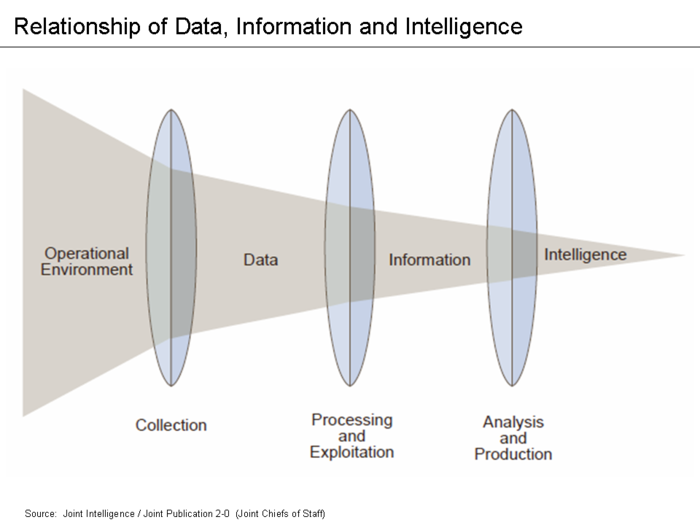
\includegraphics[scale=0.5]{DataAnalysisProcess.png} 
\caption{Here is visible a basic schema of data processes and analysis}
\end{figure}

Data analysis can be divided in some steps:

\begin{enumerate}

% 1
\item Data collection: data can be collected in a variety of ways. For example they may also be collected from sensors in the environment, such as satellites, recording devices, physical sensors etcetera. they may also be obtained through interviews, downloads from online sources, or reading documentation, so the analysis is feasible with a large variety of kinds of data. 

% 2
\item Data processing: raw data must be well-organized for analysis: for example, placing data into row, columns, vector, etcetera.

% 3
\item Data cleaning: Once pre-processed and organized, the data may be incomplete, contain duplicates, or contain errors. Data cleaning is the process of correcting these errors, eliminating duplicates and handling incomplete data. Some ways to do this are record matching (confrontation between the records to find if there is something suspicious), validation of data (if there is the sureness that data values has to respect some limits), overall quality of existing data, de-duplication (process of removing of duplications). For particular kinds of input this process is very complex (for example vocal input needs an advanced spell-checker), for others is simple (for instance online-survey interviews made using closed choices) 

% 4
\item Exploratory data analysis: in this step the data is analyzed. There are a variety of techniques referred to as exploratory data analysis to begin understanding the real content of the data. This process may result in Descriptive statistics, such as the calculation of average or median, or in Data visualization, that allows to examine the data in graphical format, through graphics and other graphical objects.

% 5
\item Modeling and algorithms: another step is using mathematical models to find relations between different variables, such as causality or correlation. An example is the regression analysis.

% 6
\item Communication: this is the final step, and it is absolutely not trivial. Is important to find a way to report the obtained information to the user in an understandable format. The communication must be adapted to the different users,  and to their requirements, to allow the data analysis to match them. 

\end{enumerate}

\section{What a user can obtain from the data?}

An user can benefit from the analysis of big data in various ways, in particular a working data analysis software can perform the subsequent tasks:

\begin{enumerate}

% 1
\item Retrieve Value: the system receives in input some cases (for instance case-A, case-B etcetera) and a set of variables (for instance variable-A, variable-B etcetera), and can shows in output the values of the variables in the set in the data cases (in case-A, case-B, variable-A = x, variable-B = y).

% 2 
\item Filter: the system can show only the subset of the data that respect some conditions.

%3
\item Find extremums, ranges and characterize distribution: the system can show the maximums o minimums values in the datasets, and in how large is the range in that the values are distributed. It is also possible to approximate with mathematical functions the statistical distributions of subsets of data 

%4 
\item Find Anomalies: check the dataset to find if there are some exceptional values, that are source of interest and need an explanation (errors in the data? unknown phenomena?)

%5
\item Clustering: the analysis is extremely easier if is possible to group different subset of data with similar characteristics. For example: in a market research, obtaining a correct clustering on the customer allows to understand the different categories of customer with different goals and needs      

\end{enumerate}

\section{Relevance in the modern market}

todoooo

\section{Root - Physical Data Analysis }

\section{Data Analysis in Aegis Experiment}

